\section*{Introduction}

This document contains the definition of the hardware configuration of the COACHES robots and the communication infrastructure. In particular, the hardware set-up of the robot is described in Section 1, the communication infrastructure in Section 2, while Section 3 illustrates the robot design.

The robots are under development by Algorithmica company\footnote{www.algorithmica.it} and they are expected to be delivered in Fall 2015.


\section{Robot Hardware Set-up}

The design of the COACHES robots has been carried out considering the requirements of the project, the environment in which they will operate, and the definition of the use cases.
Moreover, the proposed solution is based on the experience gained in building and using DIAGO robot\footnote{https://sites.google.com/a/dis.uniroma1.it/diago} at Sapienza University.

In this section, we report the main hardware components of the robot and their connections.


\subsection{Robot Hardware}

Each robot will be assembled by using the following main components.
The design of the robot is described in a later section in this document.


\subsubsection{Robot base}
The main robotic platform consists of a Segway's RMP210, shown in Fig. \ref{fig:segway}.
It is a non-balancing platform with two propulsion wheels which can operate stably in indoor environments via a third caster wheel. The base is able to load up to 45 kg, suitable to carry out the transportation tasks of the use cases defined in deliverable D5.2. Below, we describe the main technical characteristics of the platform:

\begin{table}[h]
\begin{center}
\begin{tabular}{|c|c|}
\hline 
& \bf{Segway RMP210}\\
\hline \bf{Dimensions } & 625 mm x 637 mm x 481 mm \\
\hline \bf{ Weight } & 52 kg \\
\hline \bf{ Max payload } & 45 kg \\
\hline \bf{ Max speed } & 8 m/s \\
\hline \bf{ Battery type } & LiFePO$_4$ \\
\hline \bf{ Battery capacity } & 380 Wh \\
\hline \bf{ Battery charge time } & 2-3 hours \\
\hline \bf{ Run time } & Up to 24 hours \\
\hline
\end{tabular}
\end{center}
\caption{Segway RMP210 mobile platform specifications.}
\end{table}

\begin{figure}[h!]
\begin{center}
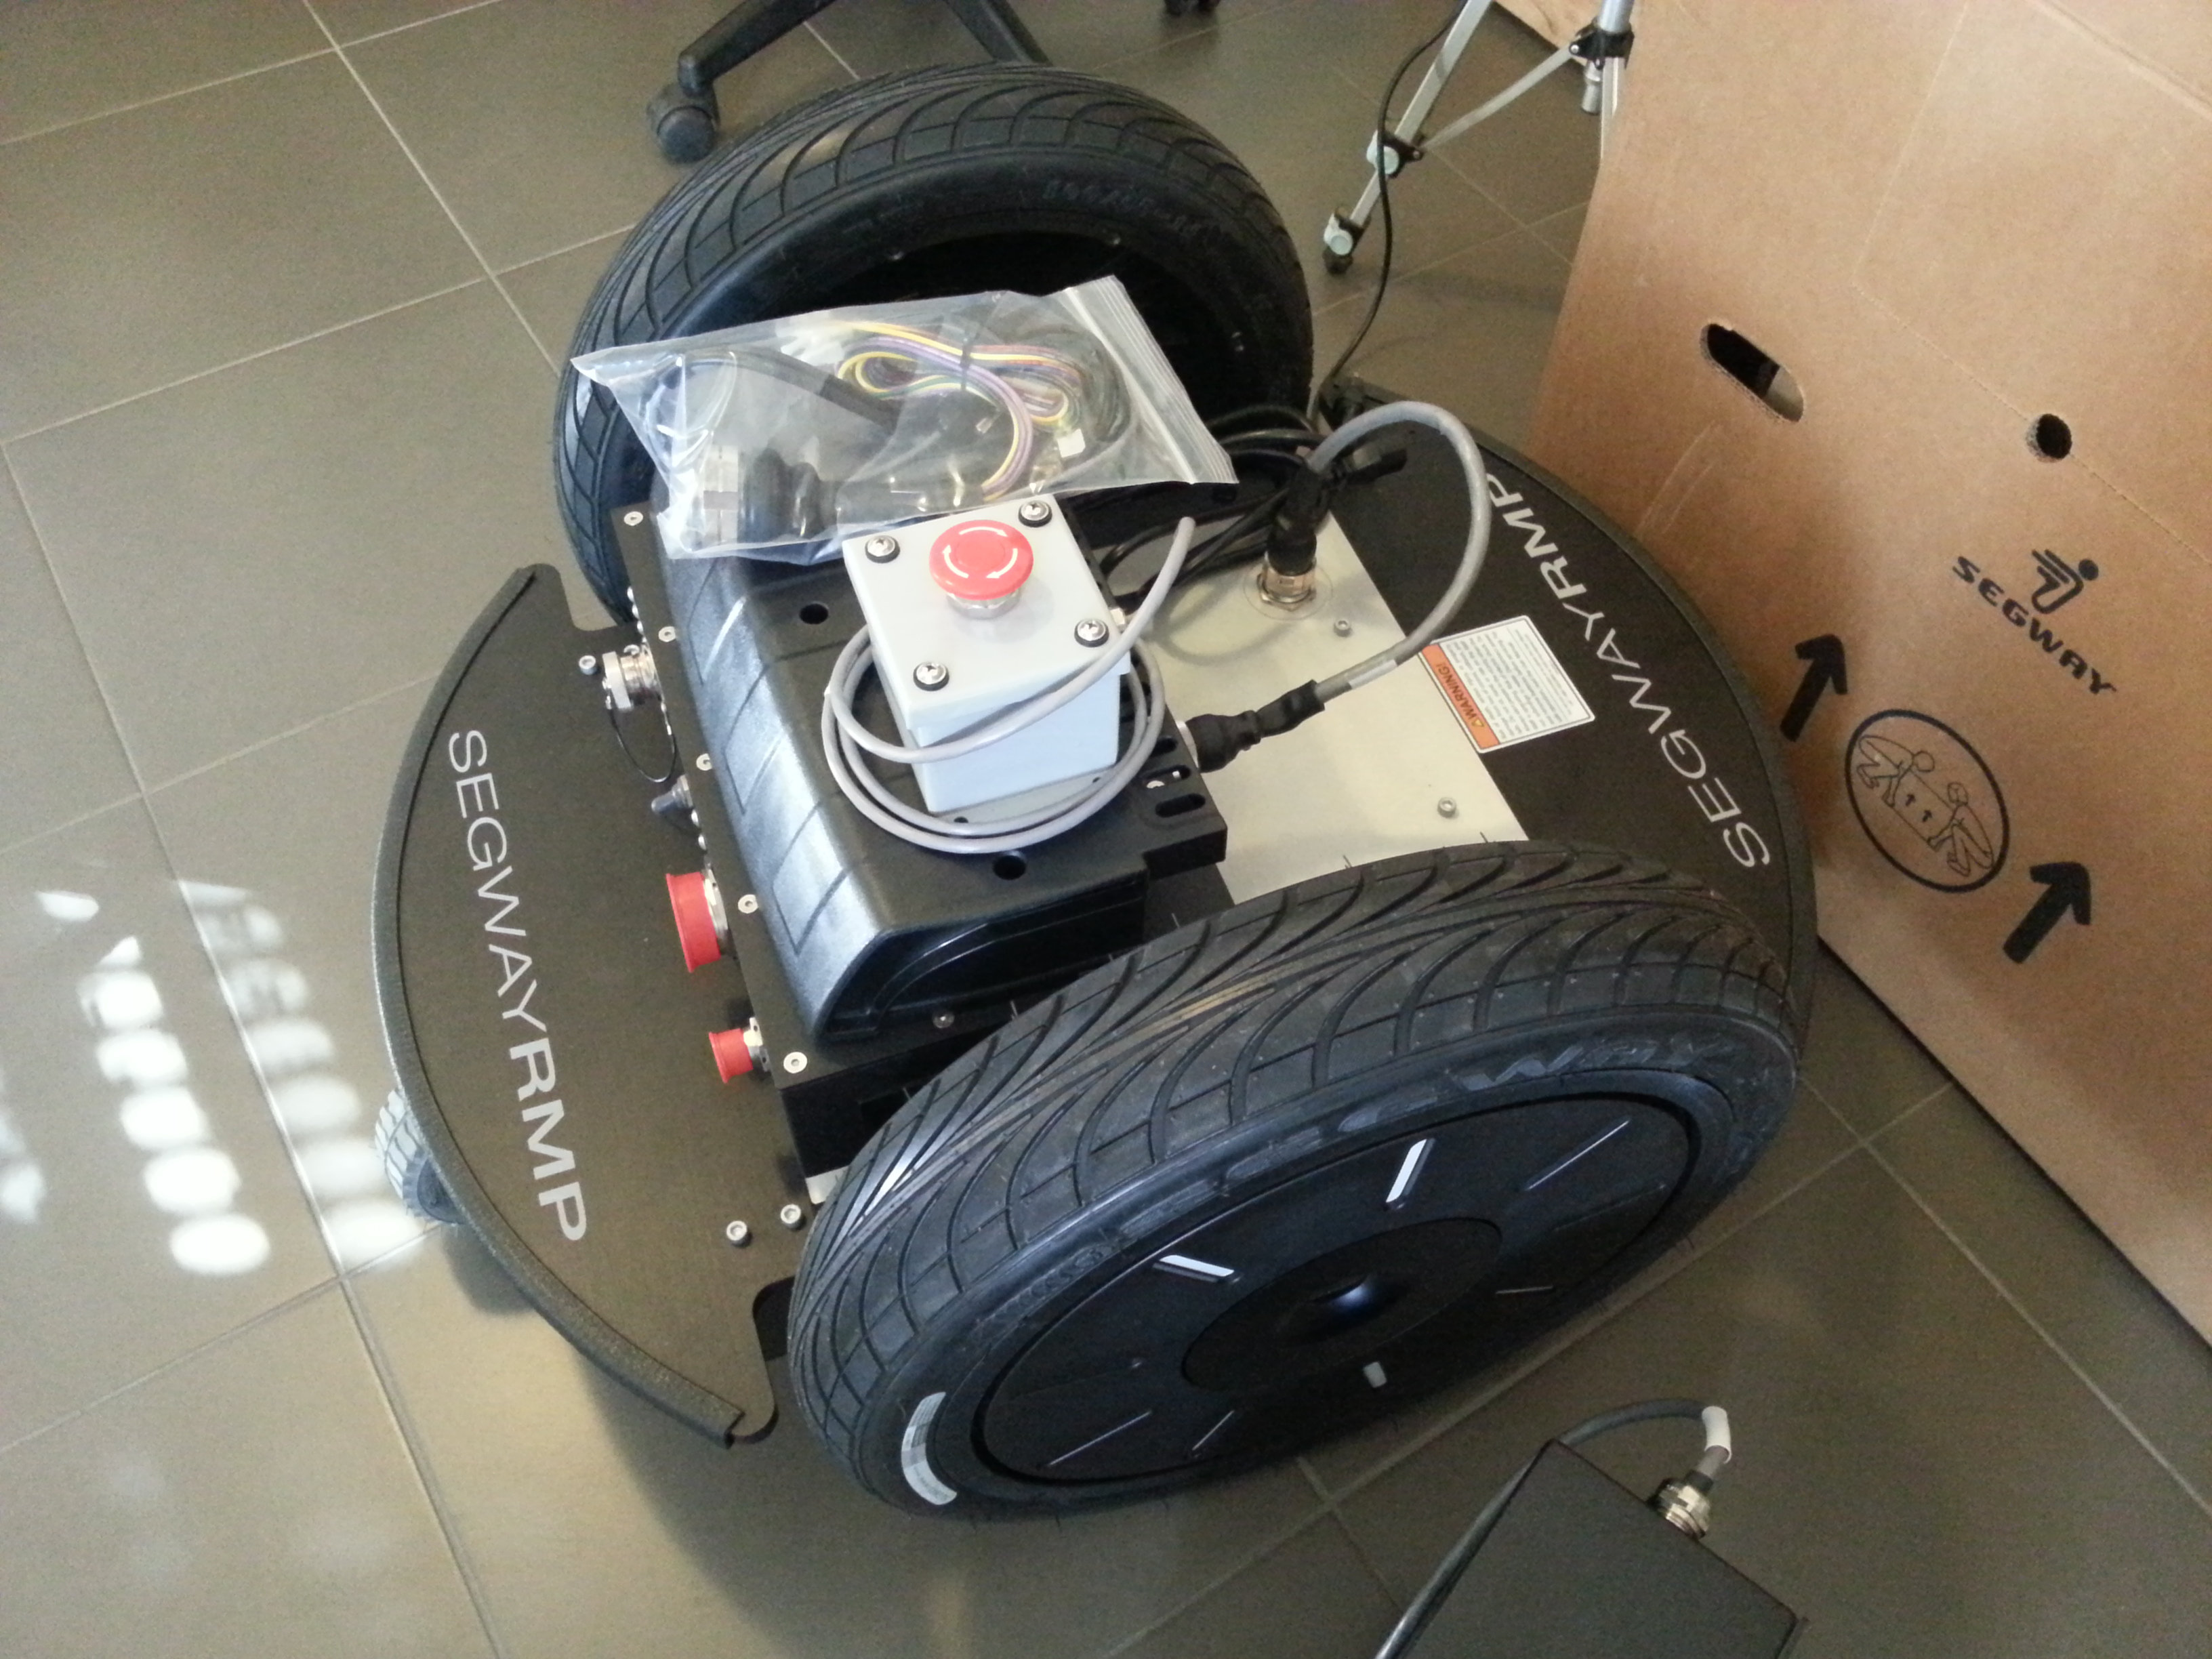
\includegraphics[height=5cm]{fig/segway_rmp210.jpg}
\end{center}
\caption{Segway RMP210 mobile platform.}
\label{fig:segway}
\end{figure}

\subsubsection{On-board sensors}

{\bf Laser range finders.} Two laser range finders equipped on the
front (Hokuyo UTM-30-LX) and back (Hokuyo URG-04LX-UG01) sides of the
robot will be used for robot localization, obstacle avoidance and
potentially people tracking.

Their specifications are summarized in the following table:

\begin{table}[h]
\begin{tabular}{|c|c|c|}
\hline \bf{Model No.}& \bf{UTM-30-LX} & \bf{URG-04LX-UG01} \\
\hline \bf{Power source} & 12VDC±10\% & 5VDC±5\%(USB Bus power) \\
\hline \bf{Detection Range} & 0.1 to 30m (Max. 60m) & 20 to 5600mm \\
\hline \multirow{2}{*}{\bf{Accuracy}}
& 0.1 to 10m: $\pm$30mm  & 60 to 1,000mm: $\pm$30mm \\
& 10 to 30m: $\pm$50mm & 1,000 to 4,095mm: $\pm$3\% of measurement \\
\hline \bf{Scan Angle} & 270$^{\circ}$ & 240$^{\circ}$ \\
\hline \bf{Angular Resolution} & 0.25$^{\circ}$ & 0.36$^{\circ}$ \\
\hline \bf{Scan Time} & 25ms  & 100ms \\
\hline \bf{Weight} & Approx. 370g  & Approx. 160g \\
\hline
\end{tabular}
\caption{Hokuyo UTM-30-LX and URG-04LX-UG01 specifications.}
\end{table}

{\bf would be interesting to know which is the actual scanning angle due to the cover.}

\begin{figure}[h!]
\begin{center}
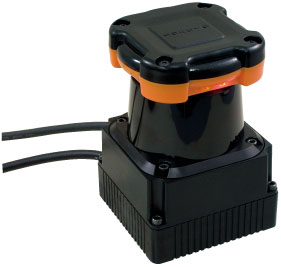
\includegraphics[height=4cm]{fig/utm30lx.jpg}
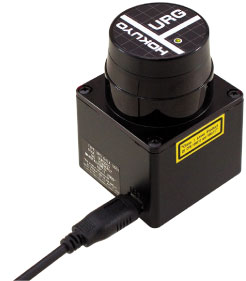
\includegraphics[height=4cm]{fig/urg04lxug01.jpg}
\end{center}
\caption{Hokuyo UTM-30-LX and URG-04LX-UG01 laser range finders.}
\label{fig:laserscans}
\end{figure}

{\bf Cameras.} The robot is mounted with 3 ASUS Xtion pro Live, a RGB
and Depth sensor that will be used for user gesture recognition,
people detection and tracking or detection of obstacles not visible by
the laser range finders. They will be arranged as it will be shown in
Section 3. 

Additionally, a Logitech HD Pro Webcam C920 is intended to be used for
robot localization in a later stage.  The camera will point to the ceiling
to take advantage of the special pattern (see Fig. \ref{fig:ceiling}) present in
the Rives de l'Orne mall, where the project demonstrations will be
carried out.

\begin{figure}[h!]
\begin{center}
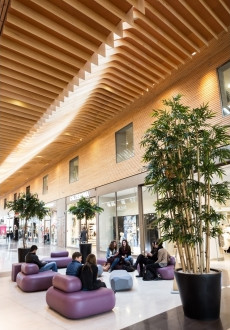
\includegraphics[height=4cm]{fig/ceiling.jpg}
\end{center}
\caption{Ceiling of the Rives de l'Orne shopping center.}
\label{fig:ceiling}
\end{figure}

\begin{figure}[h!]
\begin{center}
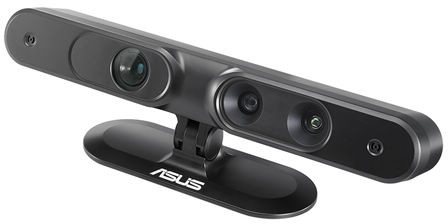
\includegraphics[height=4cm]{fig/asusxtionprolive.jpg}
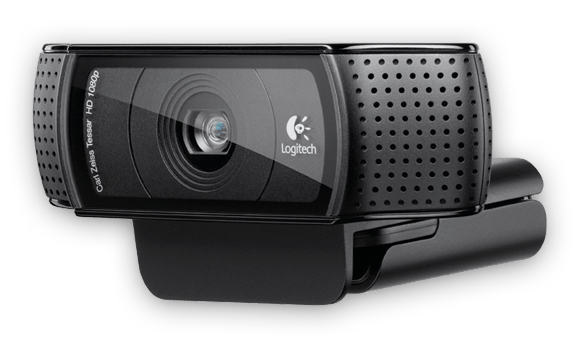
\includegraphics[height=4cm]{fig/logitech-hd-pro-webcam-c920.png}
\end{center}
\caption{ASUS Xtion pro Live and Logitech HD pro Webcam C920.}
\label{fig:cameras}
\end{figure}

\begin{table}[h]
\begin{center}
\begin{tabular}{|c|c|}
\hline
& \bf{ASUS Xtion pro Live} \\
\hline \bf{ Power Consumption } & Below 2.5W \\
\hline \bf{ Distance of Use } & Between 0.8m and 3.5m \\
\hline \bf{ Field of View } & 58° H, 45° V, 70° D (Horizontal, Vertical, Diagonal) \\
\hline \multirow{2}{*}{\bf{ Depth Image Size }} 
& VGA (640x480) : 30 fps\\
& QVGA (320x240): 60 fps \\
\hline \bf{ Resolution } & SXGA (1280*1024)  \\
\hline \bf{ Interface } & USB 2.0 (USB 3.0 Ready) \\
\hline \bf{ Dimensions } & 18 cm x 3.5 cm x 5 cm \\
\hline
\end{tabular}
\end{center}
\caption{ASUS Xtion pro Live specifications.}
\end{table}

\begin{table}[h]
\begin{center}
\begin{tabular}{|c|c|}
\hline
& \bf{Logitech HD Pro Webcam C920} \\
\hline \bf{Resolution } & Full HD video (up to 1920 x 1080 pixels) \\
\hline \bf{Video compression } & H.264 \\ 
\hline \bf{Interface } & USB 2.0 (USB 3.0 ready) \\
\hline \bf{Dimensions } & 29 mm x 24 mm x 24 mm \\ 
\hline \bf{Weight } & 162 g \\
\hline \multirow{2}{*}{\bf{Others}}
& Logitech Fluid Crystal™ Technology \\
& Carl Zeiss lens with 20-step autofocus \\
& Automatic low-light correction \\
\hline
\end{tabular}
\end{center}
\caption{Logitech HD Pro Webcam C920 specifications.}
\end{table}

\subsubsection{Human-Robot Interfaces}
Interaction with the user will be mainly through a Graphical User
Interface (GUI) displayed on a tablet Microsoft Surface Pro 2.
Although this device already incorporates stereo speakers and a
microphone, additional built-in speakers are mounted on the robot
structure and an external microphone will be used to receive commands
and spoken requests from the user. Concretely, a RODE NTG-2
professional microphone has been chosen for its capability to
eliminate the surrounding noise and focus audio recording from the main direction it is pointing to
as it is shown in Fig. \ref{fig:microphone}.
Below, we describe the main technical specifications of these devices.

\begin{table}[h]
\begin{center}
\begin{tabular}{|c|c|}
\hline
& \bf{Microsoft Surface Pro 2} \\
\hline \bf{Software} & Windows 8.1 Pro \\
\hline \bf{Dimensions} & 27.46 cm x 17.30 cm x 1.35 cm \\
\hline \bf{Weight} & 907g \\
\hline \bf{Storage} &  64/128GB/256/512GB \\
\hline \bf{Memory} & 4GB RAM  /    8GB RAM \\
\hline \multirow{3}{*}{\bf{Display}}
& Screen: 10.6 inch ClearType Full HD Display \\
& Resolution: 1920 x 1080 \\
& Touch: 10-point multi-touch \\
\hline \bf{CPU}  & 4th generation Intel® Core™ i5 Processor \\
\hline \multirow{2}{*}{\bf{Wireless Connections}} 
& Wireless: Wi-Fi (802.11a/b/g/n) \\
& Bluetooth 4.0 Low Energy technology \\
\hline \multirow{2}{*}{\bf{Camera, Video \& Audio}}  
& Two 720p HD cameras, front and rear-facing \\
& Microphone and Stereo speakers \\
\hline \multirow{3}{*}{\bf{Ports}} 
& Full-size USB 3.0 \\
& microSDXC card reader \\
& Headset jack \\
\hline \multirow{4}{*}{\bf{Sensors}}
& Ambient light sensor \\
& Accelerometer \\
& Gyroscope \\
& Magnetometer \\
\hline
\end{tabular}
\end{center}
\caption{Microsoft Surface Pro 2 specifications.}
\end{table}

\begin{table}[h]
\begin{center}
\begin{tabular}{|c|c|}
\hline
& \bf{Microphone RODE NTG-2} \\
\hline \bf{Acoustic Principle } & Line plus gradient \\
\hline \bf{Directional Pattern } & Super-Cardioid (see Fig. \ref{fig:microphone}) \\
\hline \bf{Frequency Range } & 20Hz ~ 20kHz selectable \\
\hline \bf{Output Impedence } & 250$\Omega$ \\
\hline \bf{Maximum SPL } & 131dB (@ 1kHz, 1\% THD into 1k$\Omega$ load) \\
\hline \bf{Maximum Output Level } & 6.9mV \\
\hline \multirow{2}{*}{\bf{Sensitivity}} 
& -36dB re 1 Volt/Pascal (15mV @ 94dB SPL) \\
& $\pm$2dB @ 1kHz \\
\hline \bf{Equivalent Noise } & 18dB-A SPL \\
\hline \bf{Power Requirement } & Phantom P48 or 1.5V Alkaline ‘AA’ Battery \\
\hline \bf{Output Connection } & 3-pin XLR Output \\
\hline \bf{Dimensions } & 280 mm x 22 mm x 22 mm \\
\hline \bf{Net Weight } & 161g \\
\hline
\end{tabular}
\end{center}
\caption{Microphone RODE NTG-2 specifications.}
\end{table}

\begin{figure}[h!]
\begin{center}
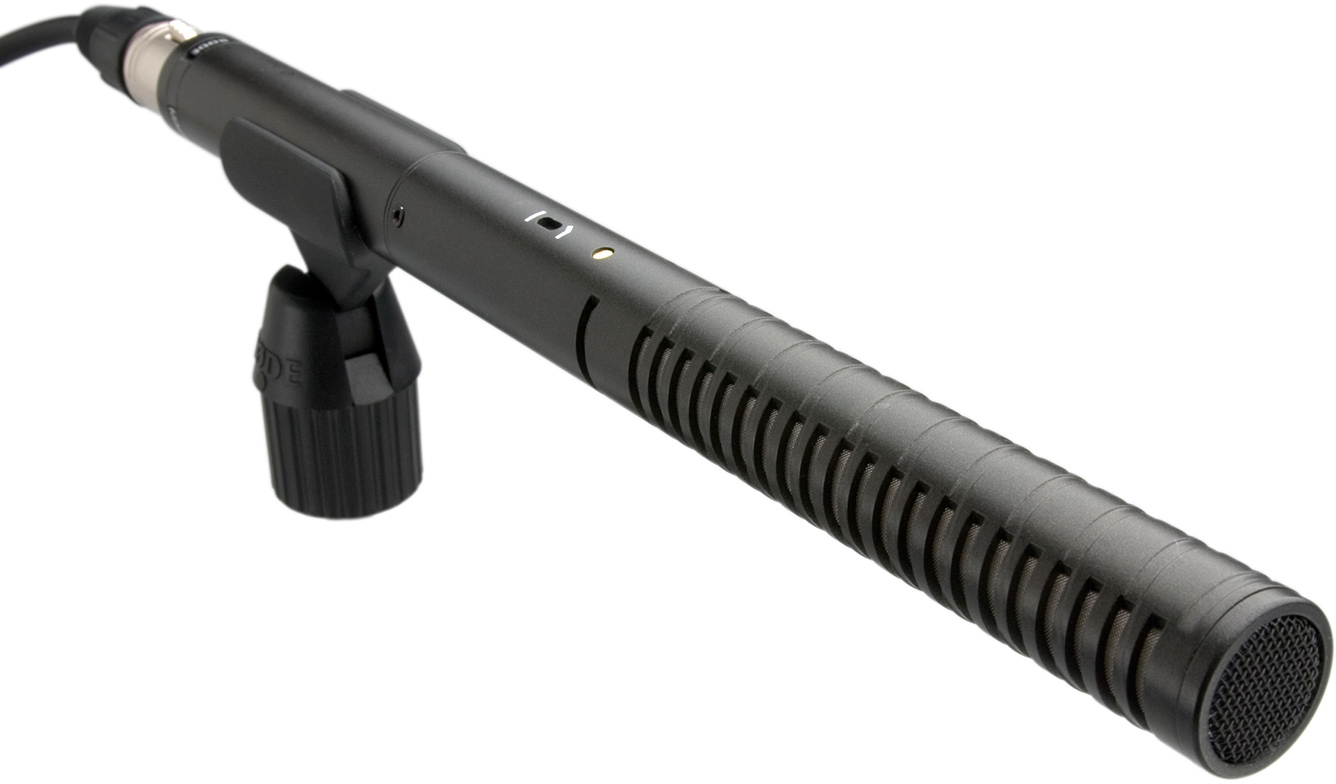
\includegraphics[height=4cm]{fig/ntg2.jpg}
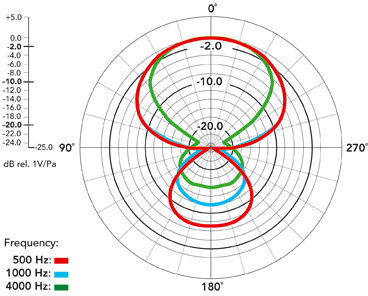
\includegraphics[height=4cm]{fig/ntg2polar.jpg}
\end{center}
\caption{Microphone RODE NTG-2 and polar pattern.}
\label{fig:microphone}
\end{figure}



\subsubsection{Additional devices}
PC laptop: HP EliteBook 820 G2
SBC: 3 Odroid C1
Network switch for internal communication and external wireless communication




\subsection{Device Connections}

Robot, 2 Laser, 3 Cameras -USB- 2 Bananas

3 Odroid  -Ethernet- Net Switch

Laptop, Tablet -Ethernet- Net Switch

Microphone -USB- Tablet

Speakers -audio jack- Tablet

External devices -Wireless- Net switch



\subsection{Device drivers}

thin\_drivers ...






